\section{はじめに}

この文章は、\cite{grisetti2010}などのチュートリアルを見ても数式の細かいところが分からない
graph-based SLAMについて、
実際の計算方法を細かく解説するためのものである。
実装例はGitHubの\texttt{ryuichiueda/probrobo\_practice}
の\texttt{./graph-based\_SLAM/graph-based\_slam.ipynb}にあり、
この文章はこの実装の数学的な解説となる。
ただし、コードで使った記号と本文章の記号は一部異なる。

\section{問題}

%対向二輪型(その場で回転できるロボット)で、
平面上を移動し、向きを持ち、カメラでランドマーク観測ができるロボットで
graph-based SLAMを実行する方法を考える。ランドマークは環境にいくつか存在し、
ロボットからは互いに識別でき、距離と見える方角が観測できる。
また、2つの観測がどの方角から観測されたものか、相対的に分かるものとする。

\subsection{ロボットの姿勢と座標系}\label{sub:pose}

世界座標系$\Sigma_\text{w}$におけるロボットの姿勢(位置と向き)を
\begin{align}
	\V{x} =
	\begin{bmatrix}
		x \\ y \\ \theta
	\end{bmatrix}
\end{align}
で表す。また、$[x\ y]^T$を原点として、$X$軸が世界座標系で$\theta$の方向を向いているロボット座標系
$\Sigma_\text{r}$を考える。これらの関係を図\ref{fig:coordinate}に示す。

\begin{figure}[htbp]
	\begin{center}
		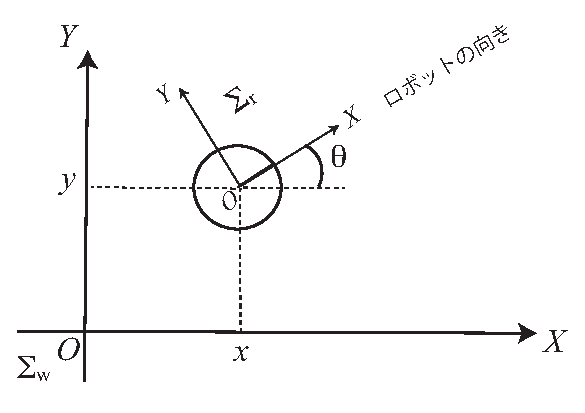
\includegraphics[width=0.5\linewidth]{./figs/coordinate.eps}
		\caption{世界座標系とロボットの姿勢}
		\label{fig:coordinate}
	\end{center}
\end{figure}

%\subsection{ロボットの運動}

離散的な時刻$t = 0,1,2,\dots,T$を考える。
時刻の集合を$\mathcal{T}$で表す。
時刻$t$における世界座標系でのロボットの姿勢を$\V{x}_t$で表す。
ロボットはデッドレコニングで$\V{x}_t$の推定値$\hat{\V{x}}_t$を認識するが、
ロボットの動作は雑音の影響を受けるため、
$\V{x}_t$と$\hat{\V{x}}_t$の間には誤差が発生する。


ロボットは一つの行動ごとに$\hat{\V{x}}_t$を記録していく。
全時刻の推定姿勢を
\begin{align}
\hat{\V{x}}_{0:T} = \{\hat{\V{x}}_0, \hat{\V{x}}_1, \dots, \hat{\V{x}}_T \}
\end{align}
と表すこととする。

\subsection{観測}

環境中にいくつかランドマークが存在していると仮定する。
時刻$t$におけるロボット座標系$\Sigma_\text{r}$を$\Sigma_{\text{r}t}$と表すこととすると、
ロボットには、時刻$t$において、全ランドマークのうちいくつかを計測する。

\subsubsection{ランドマークの識別}

ロボットからは、一度観測したランドマークは、後の時刻で観測したときに、どのランドマークか
識別できることとする。ロボットは観測したランドマークにIDを与えて管理することにする。
IDは$c$と表し(番号でも文字列でもなんでも良い)、IDとして$c$を与えられたランドマークを
$L_c$と表す。
ロボットが認識しているランドマークのIDの集合を$C$で表す。

\subsubsection{ランドマークの姿勢計測}

ロボットは$\Sigma_{\text{r}t}$においてランドマーク$L_c$を観測したとき、
$L_c$までの距離$d_{c,t}$と、ランドマークが見える方向$\varphi_{c,t}$を計測値として得る。
また、ランドマークも方角を持ち(ロボットの$\theta$に相当)、
ロボットに対してどの方角を向いているか分かることとする。
この値を$\psi_{c,t}$とする\footnote{この仮定は実用上強すぎるが、
実際には、後の計算式から分かるように、
2つの姿勢間での値$\psi_{c,t}, \psi_{c,t'}$の差だけが分かれば良い。
例えば、2点間で得られた画像の向きを画像処理から割り出すなどの処理で、この差は得られる。}。
図\ref{fig:observation}にこれらの記号の関係を示す。

\begin{figure}[htbp]
	\begin{center}
		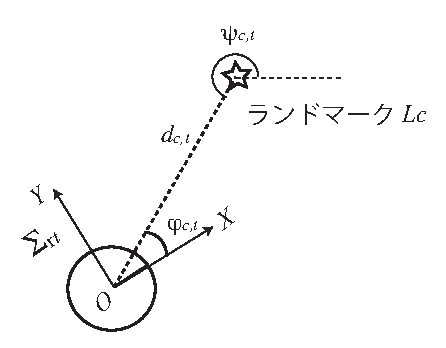
\includegraphics[width=0.5\linewidth]{./figs/observation.eps}
		\caption{計測値}
		\label{fig:observation}
	\end{center}
\end{figure}

\subsubsection{計測値の記録}

ロボットが時刻$t$で得るランドマーク全ての計測値の集合は、
$Z_t = \{ \V{z}_{c,t} = (d_{c,t}, \varphi_{c,t}, \psi_{c,t}) |
c \in C, c\text{: 観測したランドマークのID} \}$
で表すことができ、これもロボットは各時刻ごとに記録する。
$Z_t$の集合を$Z_{0:T}$で表す。

\subsubsection{計測値の誤差}\label{sub:noise}

ランドマーク観測から得られる計測値には正規分布に従う雑音が混入すると仮定する。
また、ロボットは雑音の傾向を知っていることとする。

$d_{c,t}$には、10[\%]の雑音が混入する\footnote{$「10$[\%]」は変数にすべきだが、
記号が増えて理解の妨げになるので固定値として説明する。}。
正確には真値を$d_{c,t}^*$とすると、
\begin{align}
	d_{c,t} \sim \mathcal{N}\left(d_{c,t}^*,(d_{c,t}^*/10)^2\right)
\end{align}
にしたがって$d_{c,t}$が生成される。ここで$\mathcal{N}(\mu,\sigma^2)$は
平均値$\mu$、標準偏差$\sigma$の正規分布を表す。

また、$\varphi_{c,t},\psi_{c,t}$にも$3\pi/180$[rad]の標準偏差で雑音が混入する。
これらの真値をそれぞれ$\varphi_{c,t}^*,\psi_{c,t}^*$とすると、
$\varphi_{c,t},\psi_{c,t}$は、
\begin{align}
	\varphi_{c,t} \sim \mathcal{N}\left(\varphi_{c,t}^*,(3\pi/180)^2\right) \\
	\psi_{c,t} \sim \mathcal{N}\left(\psi_{c,t}^*,(3\pi/180)^2\right)
\end{align}
で生成される。


\subsection{完全SLAM問題}

ここで、$Z_{0:T}$から、推定値$\hat{\V{x}}_{0:T}$を
真値$\V{x}_{0:T}$に近づける最適化問題を考える。
最適化のための評価関数については後述する。

\section{graph-based SLAMの実装例}

実装の一例を示す。

\subsection{グラフのエッジを作る}

問題を解くために、次のノード(頂点)、エッジ(辺、アーク)を持つグラフを考える。
\begin{itemize}
	\item ノードの持つデータ: 各時刻のロボットの推定姿勢$\hat{\V{x}}_{0:T}$
	\item エッジの持つデータ: 同じランドマーク$L_c$を観測した任意の2つの時刻$t,t'$のペアに対し、
		ランドマークの計測値から計算した観測地点間の相対姿勢$\V{\mu}_{c,t,t'}$と、
		$\V{\mu}_{c,t,t'}$に混入している雑音の共分散行列$\Sigma_{c,t,t'}$
\end{itemize}
$\V{\mu}_{c,t,t'}$、$\Sigma_{c,t,t'}$は世界座標系で定義される。

ノードのデータはデッドレコニングのデータ$\hat{\V{x}}_{0:T}$を初期値とする。一方、
エッジのデータはランドマークの計測値や、\ref{sub:noise}項で述べた値から計算する必要がある。

\subsubsection{$\V{\mu}_{c,t,t'}$の計算}

2つの時刻$t,t'$で同じランドマーク$L_c$を観測したときのロボットとランドマークの
幾何的な関係を図\ref{fig:two_poses}に示す。
二つの観測を図の点線の矢印のように世界座標系にベクトルとして描くと、
時刻$t$の観測のベクトルに、時刻$t'$の観測のベクトルの
向きを反転して足せば$\V{\mu}_{c,t,t'}$が求まることが分かる。


\begin{figure}[htbp]
	\begin{center}
		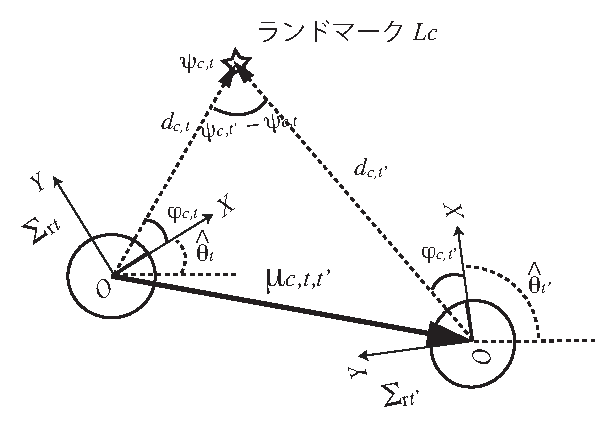
\includegraphics[width=0.5\linewidth]{./figs/two_poses.eps}
		\caption{ランドマークの計測値から2点の相対姿勢を求める}
		\label{fig:two_poses}
	\end{center}
\end{figure}

したがって、$\V{\mu}_{c,t,t'}$($x,y,\theta$座標のベクトルとなる)
は次のような単純な幾何計算で求まる
\footnote{おそらく$\psi$は$\hat\theta$で置き換えられるので
$\psi$を使わない実装もできるが、まだ自分自身では検証していない。}。
\begin{align}
	\V{\mu}_{c,t,t'} =
	\begin{bmatrix}
	d_{c,t'} \cos(\hat{\theta}_{t'} + \varphi_{c,t'}) \\
	d_{c,t'} \sin(\hat{\theta}_{t'} + \varphi_{c,t'}) \\
	\psi_{c,t'}
	\end{bmatrix}
	- 
	\begin{bmatrix}
	d_{c,t} \cos(\hat{\theta}_t + \varphi_{c,t}) \\
	d_{c,t} \sin(\hat{\theta}_t + \varphi_{c,t}) \\
	\psi_{c,t}
	\end{bmatrix}
\end{align}

\subsubsection{$\Sigma_{c,t,t'}$の計算}







